%! TEX root = ../../master.tex
\lecture[Matching-like algorithms. $T$-joins as a generalization. Properties of $T$-joins. Optimal $T$-joins in poly-time.]{Do 09 June 2022}{$T$-joins}

We know how to efficiently find optimal general matchings, implying we can also efficiently solve the separation problem
with blossom contraints.
\begin{theorem}
    There is an efficient non-Ellipsoid separation algorithm for blossom constraints.
\end{theorem}
\begin{proof}
    The algorithm can be found in \cite[Ch.~6.8]{comb-optimization-cook}. The rough idea is to use submodularity.
\end{proof}
We want to have a look at further matching-like problems.
\begin{definition}
    Given an undirected graph $G=(V,E)$. We want to find a min-cost walk traversing every edge at least once and finishing where we started.
    This problem is called \vocab{Postal Delivery Problem}, or archaically \vocab{Chinese Postman Problem}.
\end{definition}
\begin{remark}
    In the optimal case, every edge needs only to be traversed once, leading to the lower bound $\sum_{e\in E} c(e)$.
    The decision problem if this is possible is called \vocab{Euler Tour}, or historically \vocab{K\"onigsberg Bridge Problem}.
\end{remark}
\begin{fact}
    Given graph $G$. An Euler Tour exists in $G$ iff all nodes have even degree and $G$ is connected.
\end{fact}
\begin{definition}
    We call $G$ \vocab{Eulerian} if $G$ has an Euler Tour.
\end{definition}
What remains to be analyzed for the Postal Delivery Problem is the case if $G$ is not Eulerian.
For this, let $T$ be the set of nodes with odd degree.
We want to find a min-cost subset $J \subseteq E$ such that $E \uplus J$ is Eulerian,
because this $J$ can be interpreted as the edges we need to traverse twice (one can show there are optimal solutions with this property).

But in fact, nothing restricts us to let $T$ be any even subset of nodes:
\begin{definition}
    For a graph $G=(V,E)$, consider even-sized $T \subseteq V$ and $J \subseteq E$. If
    \begin{align*}
        T = \{i \in \natnum \mid \deg_J(i) \text{ is odd}\},
    \end{align*}
    we call $J$ a $T$-join.
    For an additional cost vector $c$, the corresponding optimization problem of finding a minimal $T$-join is given by
    \begin{mini*}{J}{c(J)}{}{}
        \addConstraint{J}{\text{ is $T$-join}}
    \end{mini*}
\end{definition}
\begin{remark}
    Applications of this are
    \begin{enumerate}
        \item our postal delivery problem using all odd nodes,
        \item for $T=\{s,t\}$, an optimal $T$-join is an $s-t$-path with negative costs allowed,
        \item for even $|N|$ and $T=N$, a $T$-join is a min-cost general matching.
    \end{enumerate}
\end{remark}
\begin{example}
    Let's construct a $T$-join, for $\textcolor{blue}{T=\{1,3,5,9\}}$:
    \vspace{5pt}
    \\
    \begin{minipage}{\textwidth}
        \centering
        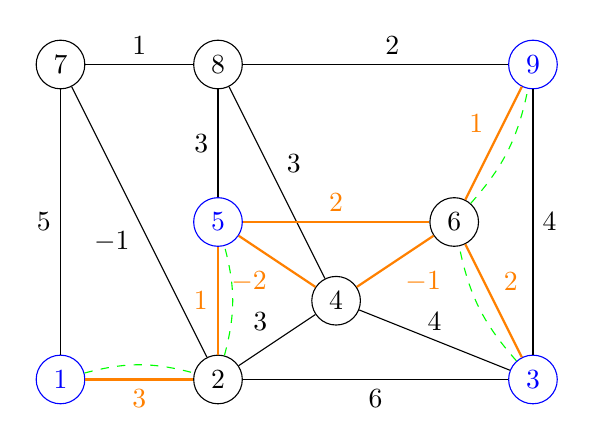
\begin{tikzpicture}
            \begin{scope}[every node/.style={circle, draw}]

                \node[blue] (1) at (0,0) {1};
                \node (2) at (2,0) {2};
                \node[blue] (3) at (6,0) {3};
                \node (4) at (3.5,1) {4};
                \node[blue] (5) at (2,2) {5};
                \node (6) at (5,2) {6};
                \node (7) at (0,4) {7};
                \node (8) at (2,4) {8};
                \node[blue] (9) at (6,4) {9};

            \end{scope}
            \path[orange, thick] (1) edge node[anchor=north] {3}(2);
            \path[green, dashed] (1) edge[bend left=15]  (2);
            \path (1) edge node[anchor=east] {5}(7);
            \path (2) edge node[anchor=north] {6}(3);
            \path (2) edge node[anchor=south east] {3}(4);
            \path[orange, thick] (2) edge node[anchor=east] {1}(5);
            \path[green, dashed] (2) edge[bend right=15]  (5);
            \path (2) edge node[anchor=north east] {$-1$}(7);
            \path (3) edge node[anchor=south] {4}(4);
            \path[orange, thick] (3) edge node[anchor=south west] {2}(6);
            \path[green, dashed] (3) edge[bend left=15]  (6);
            \path (3) edge node[anchor=west] {4}(9);
            \path[orange, thick] (4) edge node[anchor=north east] {$-2$}(5);
            \path[orange, thick] (4) edge node[anchor=north west] {$-1$}(6);
            \path (4) edge node[anchor=south west] {3}(8);
            \path[orange, thick] (5) edge node[anchor=south] {2}(6);
            \path (5) edge node[anchor=east] {3}(8);
            \path[orange, thick] (6) edge node[anchor=south east] {1}(9);
            \path[green, dashed] (6) edge[bend right=15]  (9);
            \path (7) edge node[anchor=south] {1}(8);
            \path (8) edge node[anchor=south west] {2}(9);

        \end{tikzpicture}
    \end{minipage}
    Then the \textcolor{orange}{orange edges $J$} form a \textcolor{blue}{$T$-join},
    but while cheaper, this isn't minimal like the \textcolor{green}{green edges $J'$}.
\end{example}
\begin{theorem}
    If $J$ is a minimal (w.r.t.\ to its choice of edges) $T$-join, then $J$ is a collection of $|T|/2$ edge-disjoint paths.
\end{theorem}
\begin{proof}
    We prove by induction over even size $|J|$. Base case $0$ is trivial.
    Consider $t \in T$ and let $C$ be a connected component of $(V,J)$ cont.t.
    Note $\delta_J(t)$ is odd, and $\sum_{i\in C}\delta_J(i)$ is even, therefore there exists
    another $s \in C$ with $\delta_J{s}$ odd.
    By removing $\{s,t\}$ from $T$ and the $s-t$-path from $J$, we keep our $T$-join property, enabling us to use our induction step.
\end{proof}
\begin{theorem}
    Let $s,t \in T$ connected by path $P$ in a $T$-join $J$. Suppose there exists a cheaper $s-t$-path $P'$.
    Then, $J$ is not an optimal $T$-join.
\end{theorem}
\begin{proof}
    We show that
    \begin{align*}
        J' \coloneqq (J - P) \Delta P'
    \end{align*}
    is a better $T$-join. Deleting $P$ will result only in $s,t$ changing parity.
    Adding $P'$ then again changes parity of $s,t$, either by adding or deleting exactly one edge.
    For the other nodes in $P'$, either $0,1$, or $2$ edges are also in $Q$, but every case doesn't change parity again.
    So, we maintain $T$-join-property.

    Calculating everything further yields
    \begin{align*}
        c(J') & \leq c(J) + c(P' \setminus P) - c(P \setminus P')                                \\
              & = c(J) + (c(P' \setminus P) - c(P' \cap P)) - (c(P \setminus P') - c(P' \cap P)) \\
              & = c(J) + \underbrace{c(P')-c(P)}_{<0}< c(J)
    \end{align*}
    as wished.
\end{proof}
\begin{corollary}
    If $c \geq 0$, then optimal $J$ consists of $|T|/2$ shortests paths.
\end{corollary}
Consider now negative costs $c$.
\begin{definition}
    Let $M \subseteq E$ be the set of negative-valued edges, and define
    \begin{align*}
        T^M \coloneqq  \{i \in \natnum \mid \delta_M(i) \text{ is odd}\}.
    \end{align*}
\end{definition}
\begin{remark} \label{note:minus-join}
    $M$ is a $T^M$-join.
\end{remark}
\begin{lemma} \label{thm:diff-joins}
    If $J$ is a $T$-join and $J'$ is a $T'$-join, then $J \Delta J'$ is a $(T \Delta T')$-join.
\end{lemma}
\begin{proof}
    Let $v \in T \Delta T'$. Then w.l.o.g.\ $v \in T$ and $v \not \in T'$,
    so $\deg_{J}(v)$ is odd, while $\deg_{J'}(v)$ is even. Because only edges that are both in $J$ and $J'$
    cancel each other out in $J \Delta J'$, it holds $\deg_{J\Delta J'}(v) \equiv \deg_{J}(v) + \deg_{J'}(v) \equiv 1 \pmod{2}$.

    Otherwise, $v \not \in T \Delta T'$, so $v$ is either in both or none of $J, J'$.
    An analoguous argument shows $\deg_{J\Delta J'}(v) \equiv \deg_{J}(v) + \deg_{J'}(v) \equiv 0 \pmod{2}$.
\end{proof}
\begin{theorem}
    $J$ is an optimal $T$-join w.r.t.\ cost vector $c$
    iff $J \Delta M$ is an optimal $(T \Delta T^M)$-join w.r.t.\ cost vector $|c|$.
\end{theorem}
\begin{proof}
    By \autoref{thm:diff-joins} and \autoref{note:minus-join} we can form the symmetric difference of
    any side and get the other side as a corresponding join (note $A \Delta B \Delta B = A$).
    It remains to prove optimality. Calculations show:
    \begin{align*}
        c(J) & = c(J \setminus M) + c(J \cap M) + \underbrace{c(M\setminus J) - c(M\setminus J)}_{=0}                               \\
             & = \underbrace{c(J \setminus M)}_{\text{only positive}} + c(M) - \underbrace{c(M \setminus J)}_{\text{only negative}} \\
             & = |c|(J \Delta M) + c(M)
    \end{align*}
    So, minimizing one side also minimizes the other side, which immediately proves our equivalence (note $c(M)$ is constant).
\end{proof}
\begin{corollary}
    Calculating an optimal $T$-join is in $\pP$.
\end{corollary}
\begin{example}
    Building upon previous example, again consider $\textcolor{blue}{T=\{1,3,5,9\}}$,
    but note now $\textcolor{green}{T^M = \{2,5,6,7\}}$ and $\textcolor{red}{T \Delta T^M = \{1,2,3,6,7,9\}}$.
    \vspace{5pt}
    \\
    \begin{minipage}{\textwidth}
        \centering
        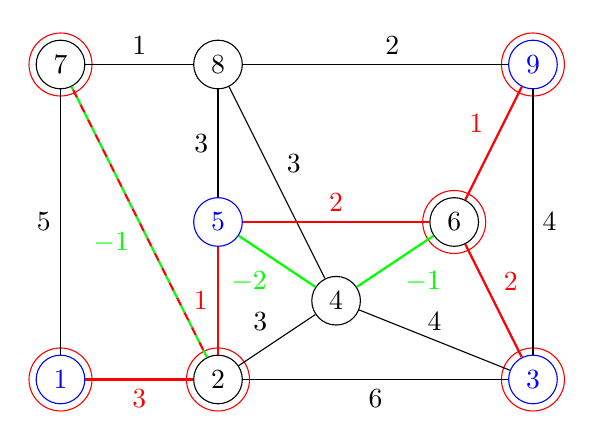
\begin{tikzpicture}
            \begin{scope}[every node/.style={circle, draw}]

                \node[blue] (1) at (0,0) {1};
                \draw[red] (0,0) circle (0.4);
                \node (2) at (2,0) {2};
                \draw[red] (2,0) circle (0.4);
                \node[blue] (3) at (6,0) {3};
                \draw[red] (6,0) circle (0.4);
                \node (4) at (3.5,1) {4};
                \node[blue] (5) at (2,2) {5};
                \node (6) at (5,2) {6};
                \draw[red] (5,2) circle (0.4);
                \node (7) at (0,4) {7};
                \draw[red] (0,4) circle (0.4);
                \node (8) at (2,4) {8};
                \node[blue] (9) at (6,4) {9};
                \draw[red] (6,4) circle (0.4);

            \end{scope}
            \begin{scope}[every edge/.style={draw,green,thick,
                            dash pattern=on 3pt off 3pt,
                            postaction={draw,red,thick,
                                    dash pattern= on 3pt off 3pt,
                                    dash phase=3pt}}]
                \path (2) edge node[anchor=north east] {$-1$}(7);
            \end{scope}

            \path[green,thick] (4) edge node[anchor=north east] {$-2$}(5);
            \path[green,thick] (4) edge node[anchor=north west] {$-1$}(6);

            \path[red,thick] (1) edge node[anchor=north] {3}(2);
            \path (1) edge node[anchor=east] {5}(7);
            \path (2) edge node[anchor=north] {6}(3);
            \path (2) edge node[anchor=south east] {3}(4);
            \path[red,thick] (2) edge node[anchor=east] {1}(5);
            \path (3) edge node[anchor=south] {4}(4);
            \path[red,thick] (3) edge node[anchor=south west] {2}(6);
            \path (3) edge node[anchor=west] {4}(9);
            \path (4) edge node[anchor=south west] {3}(8);
            \path[red,thick] (5) edge node[anchor=south] {2}(6);
            \path (5) edge node[anchor=east] {3}(8);
            \path[red,thick] (6) edge node[anchor=south east] {1}(9);
            \path (7) edge node[anchor=south] {1}(8);
            \path (8) edge node[anchor=south west] {2}(9);

        \end{tikzpicture}
    \end{minipage}
    Note that the red edges form an optimal $T \Delta T^M$-join. Taking its symmetric difference
    with $M$ directly yields our initial (optimal) $T$-join.
\end{example}
We still need an $\LP$-formulation, though. We will utilize following definition for this:
\begin{definition}
    If $S \subseteq E$ such that $|S \cap T|$ is odd (even), we call $S$ \vocab[T-odd]{$T$-odd} (\vocab[T-even]{$T$-even}).
\end{definition}
\begin{theorem}
    If $c \geq 0$, then solving
    \begin{mini*}{x}{c^Tx}{}{}
        \addConstraint{x(\delta(S))}{\geq 1, \quad}{\forall \text{ $T$-odd } S \subseteq E}
        \addConstraint{x}{\geq 0}
    \end{mini*}
    yields an optimal $T$-join.
\end{theorem}
\begin{proof}
    See \cite[Thm.~5.28]{comb-optimization-cook}.
\end{proof}
However, there are two problems:
\begin{enumerate}
    \item It is only $\frac{1}{2}$-integral and not totally dual integral.
    \item If $c$ arbitrary, then it could be unbounded.
\end{enumerate}
We can circumvent these problems with a tighter $\LP$.
Consider following motivation:
Let $S \subseteq N$ and $F \subseteq \delta(S)$.
If $S$ is $T$-odd and $|F|$ even, then $|\delta(S) \setminus F|$ is odd.
This means, if $J$ is a $T$-join and uses all edges in $F$, then it must
also use at least one edge from $\delta(S) \setminus F$.
Analoguous, if $S$ is $T$-even, we conclude $|F|$, and get to the same result.
We encode this property as follows: \todo{why is $\delta(S)$ always odd?}
\begin{theorem}
    For any $c$, the $\LP$
    \begin{mini*}{x}{c^Tx}{}{}
        \addConstraint{x(\delta(S) \setminus F)}{\geq 1 + x(F) - |F|, \quad}{\forall S,F, |S \cap T| + |F| \text{ odd}}
        \addConstraint{1 \geq x}{\geq 0}
    \end{mini*}
    is Totally Dual Integral and yields an integral optimal $T$-join.
\end{theorem}
\begin{proof}
    Note the right side is equal to 1 iff all edges of $F$ are used.
    For the actual proof, see \cite[Thm.~5.30]{comb-optimization-cook}.
\end{proof}